\documentclass[border=10pt]{standalone}

\usepackage{tikz}
\usepackage{tikzsymbols}
\usetikzlibrary{calc,patterns,shapes.geometric}

\def\centerarc[#1](#2)(#3:#4:#5){\draw[#1] ($(#2)+({#5*cos(#3)},{#5*sin(#3)})$) arc (#3:#4:#5);}

\begin{document}
	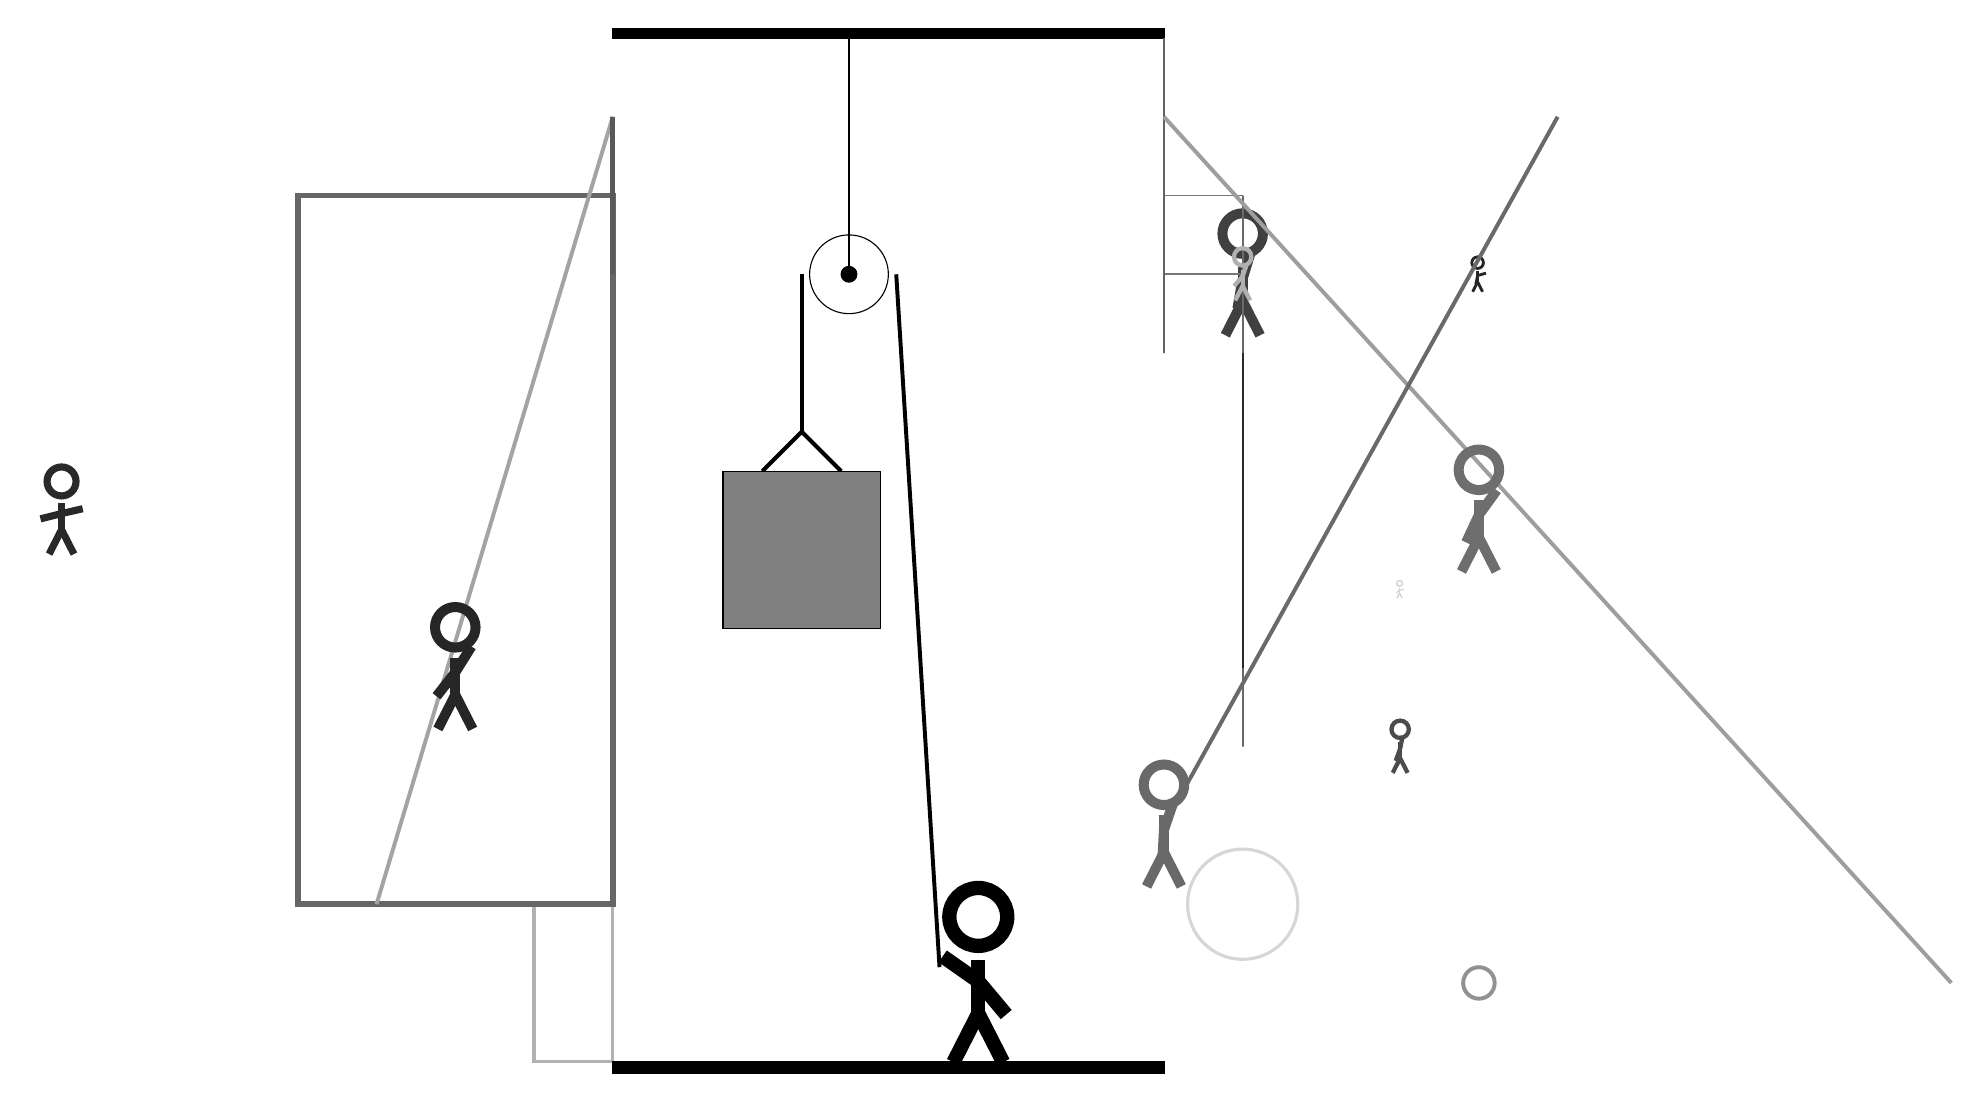
\begin{tikzpicture}
		%%%%% START %%%%%
		
		\draw[fill=black] (-2, 10) rectangle (5, 10.125);
		
		\draw (1, 7) circle (0.5);
		\draw[fill=black] (1, 7) circle (0.1);
		\draw (1, 10) -- (1, 7);
		
		\draw[line width=0.5mm] (-0.1, 4.5) -- (0.4, 5.0) -- (0.9, 4.5);
		\draw[fill=black!50] (-0.6, 4.5) rectangle (1.4, 2.5);
		
		\draw[line width=0.5mm] (0.4, 7) -- (0.4, 5.0);
		\centerarc[line width=0.5mm](1, 7)(0:180:0.6);
		\draw[line width=0.5mm](1.6, 7) -- (2.15, -1.8);
		
		\node at (2.6, -1.9) {\Strichmaxerl[10][-35][-50]};
		
		\node[line width=0.6mm, color=black!75] at (6, 7) {\Strichmaxerl[7][80][73]};
		
		\node[line width=0.7mm, color=black!85] at (9, 7) {\Strichmaxerl[2][78][16]};
		\draw[line width=0.4mm, color=black!30] (-2, -3) rectangle (-3, -1);
		\node[line width=0.3mm, color=black!17] at (8, 3) {\Strichmaxerl[1][45][5]};
		
		\draw[line width=0.2mm, color=black!53] (5, 7) rectangle (6, 8);
		\node[line width=0.3mm, color=black!70] at (8, 1) {\Strichmaxerl[3][70][79]};
		
		\draw[line width=0.2mm, color=black!61] (5, 6) rectangle (5, 10);
		\draw[line width=0.3mm, color=black!59] (6, 8) rectangle (6, 1);
		\node[line width=0.4mm, color=black!31] at (6, 7) {\Strichmaxerl[3][49][71]};
		\draw[line width=0.3mm, color=black!84] (6, 6) rectangle (6, 2);
		\draw[line width=0.7mm, color=black!60] (-2, 8) rectangle (-6, -1);
		
		\draw [line width=0.4mm, color=black!16](6, -1) circle (0.7);
		\draw [line width=0.5mm, color=black!43](9, -2) circle (0.2);
		
		\node[line width=0.6mm, color=black!84] at (-9, 4) {\Strichmaxerl[5][14][13]};
		\draw[line width=0.5mm, color=black!38](5, 9) -- (15, -2);
		\draw[line width=0.5mm, color=black!59](10, 9) -- (5, 0);
		
		\draw [line width=0.4mm, color=black!32](-2, 3) circle (0.0);
		\draw[line width=0.5mm, color=black!36](-2, 9) -- (-5, -1);
		\draw[line width=0.6mm, color=black!65] (-2, 9) rectangle (-2, 7);
		
		\node[line width=0.7mm, color=black!57] at (9, 4) {\Strichmaxerl[7][65][54]};
		\node[line width=0.2mm, color=black!59] at (5, 0) {\Strichmaxerl[7][87][71]};
		
		\node[line width=0.6mm, color=black!85] at (-4, 2) {\Strichmaxerl[7][52][58]};
		
		\draw[fill=black] (-2, -3) rectangle (5, -3.15);
		
		%%%%% END %%%%%
	\end{tikzpicture}
\end{document}